\documentclass[journal]{new-aiaa}
%\documentclass{ahs}
%\usepackage[dvips]{graphicx}
\usepackage{graphicx}
%\usepackage{amsmath}
%\usepackage{array}
%\usepackage{latexsym}
%\usepackage{cite}
\usepackage{hyperref}
\usepackage[T1]{fontenc}
\usepackage{lmodern}
%\setmainfont[Mapping=tex-text, Color=textcolor]{CMU Serif}
%\usepackage{fancyvrb}
%\usepackage{dcolumn}
% more text vertically
%\addtolength{\textheight}{0.5in}
%\addtolength{\topmargin}{-0.5in}
% more text horizontally
%\setlength{\oddsidemargin}{0.25in}
%\setlength{\evensidemargin}{0.25in}
%\addtolength{\textwidth}{0.5in}
% more closely-positioned figures
%\renewcommand{\topfraction}{0.75}
%\renewcommand{\bottomfraction}{0.5}
%\renewcommand{\textfraction}{0.25}
%\renewcommand{\floatpagefraction}{0.75}
\usepackage{longtable,tabularx}
\setlength\LTleft{0pt}
%\usepackage[nomarkers,nolists,figuresonly]{endfloat}
\usepackage[nomarkers,nolists,tablesonly]{endfloat}
%\usepackage{endfloat}
\renewcommand{\efloatseparator}{\mbox{}}

% --------------------------------------------------------------------------

\title{Robust and Corrected Coefficients for the ROBIN Body}

\author{Blake B.~Hillier\footnote{Engineering Intern}}
\author{Mark J.~Stock\footnote{Corresponding author, markjstock@gmail.com, Senior Research Scientist}}
\author{Adrin Gharakhani\footnote{President, Senior AIAA Member}}
\affil{Applied Scientific Research, Inc.\\ Irvine, CA}

\begin{document}
\maketitle

% Technical notes have no abstract

\section*{Nomenclature}

{\renewcommand\arraystretch{1.0}
\noindent\begin{longtable*}{@{}l @{\quad=\quad} l@{}}
$x,y,z$  & Cartesian coordinates \\
$C_{i}$ &    $i$-th coefficient \\
$H,W$ &    height, width coefficients \\
$N$ &    elliptical power \\
$Z0$ &    camber line \\
\end{longtable*}}

% --------------------------------------------------------------------------

\section{Introduction}
The ROBIN (ROtor-Body-INteraction) body is a VTOL fuselage shape \cite{nasa80051,nasa87762,mineckgorton,nasa1999}
defined by the intersection of multiple sets of analytic equations.
This shape is very useful as a benchmark for rotorcraft aerodynamics research, but the formulae
as published will generate floating point errors during computation,
and even if those are fixed, the coefficients will not recreate a usable shape.
While subsequent authors have presented corrections \cite{nasa87762,mineckgorton},
none have reported all that are required to generate the proper shape.
\begin{figure}[b]
\begin{centering}
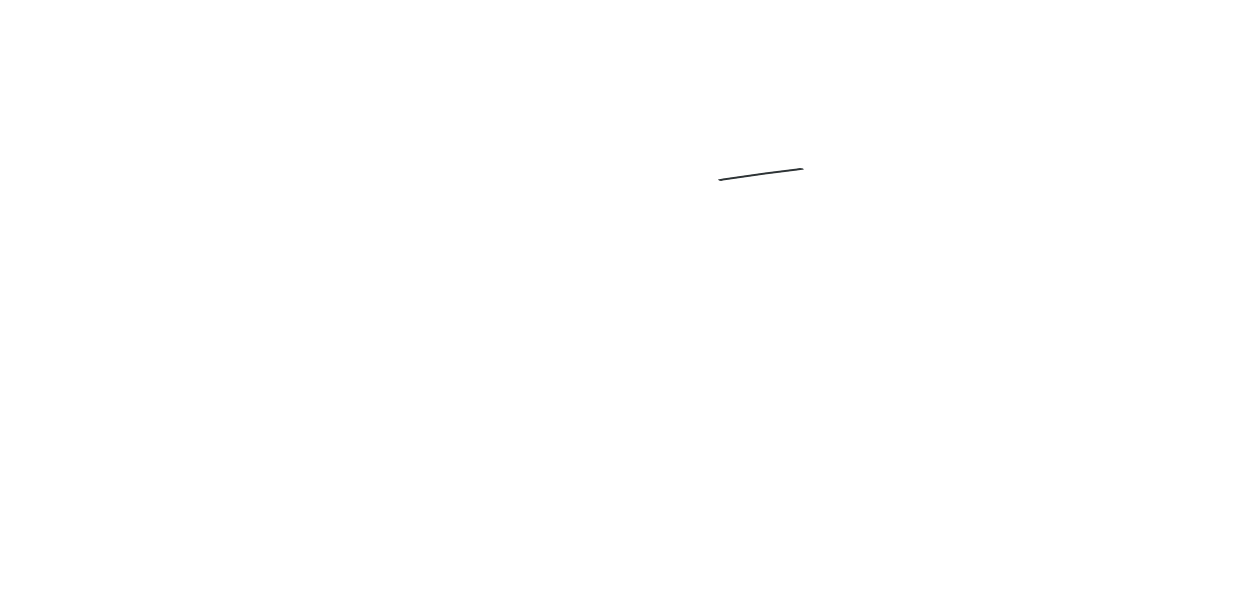
\includegraphics[width=2.1in]{img_figa.png}
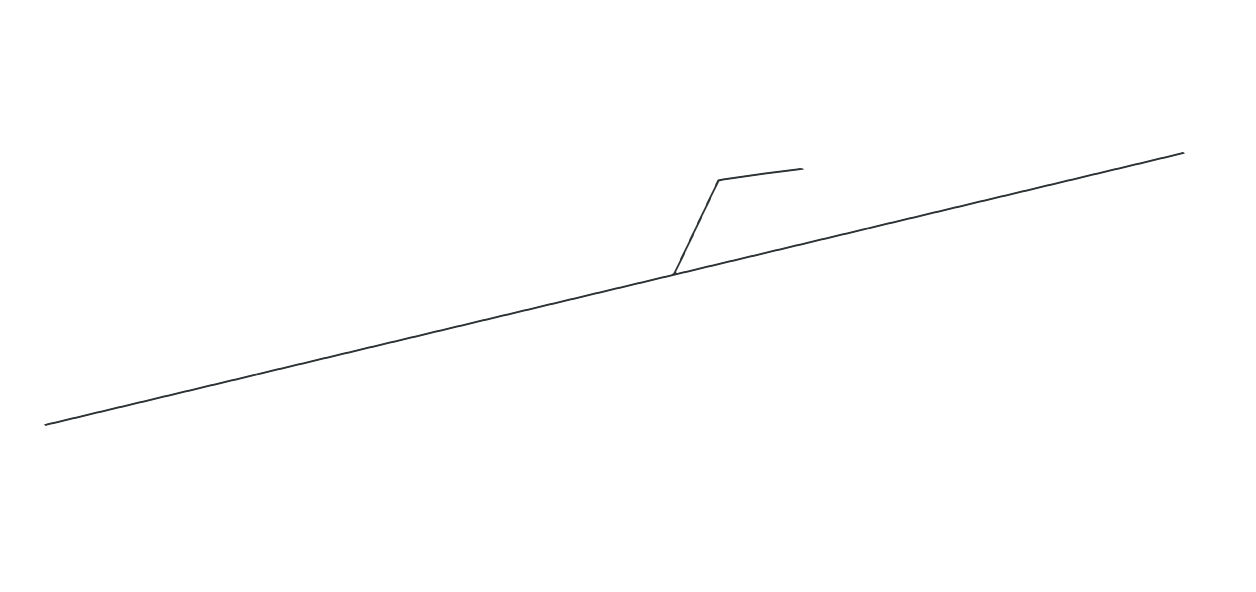
\includegraphics[width=2.1in]{img_figc.png}
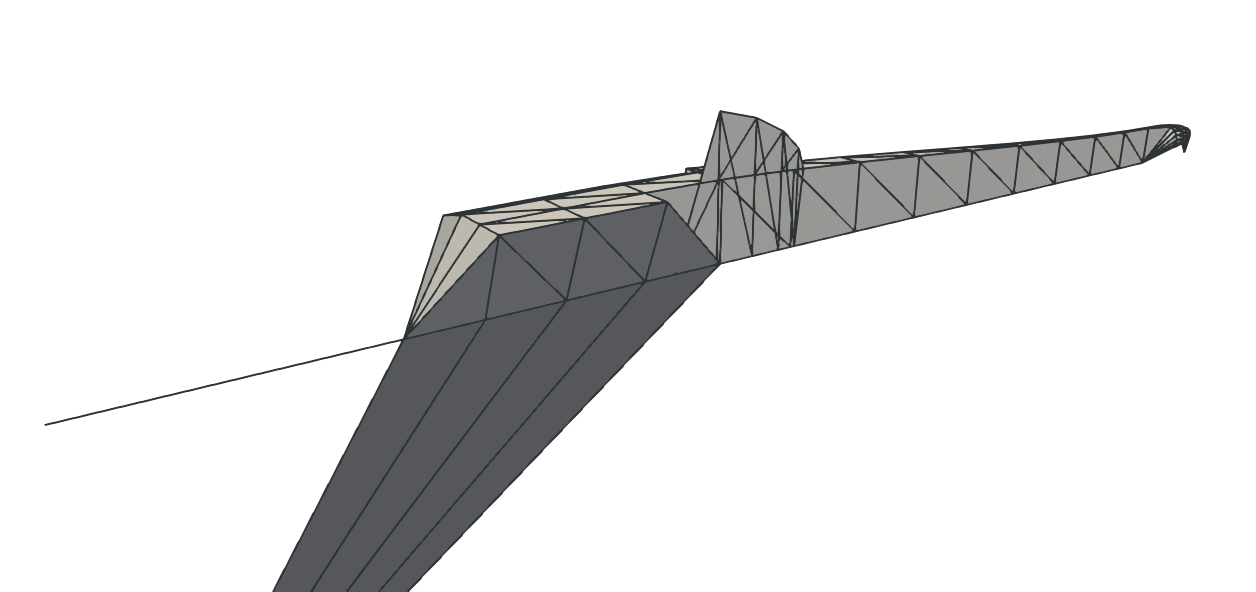
\includegraphics[width=2.1in]{img_figd.png} \\
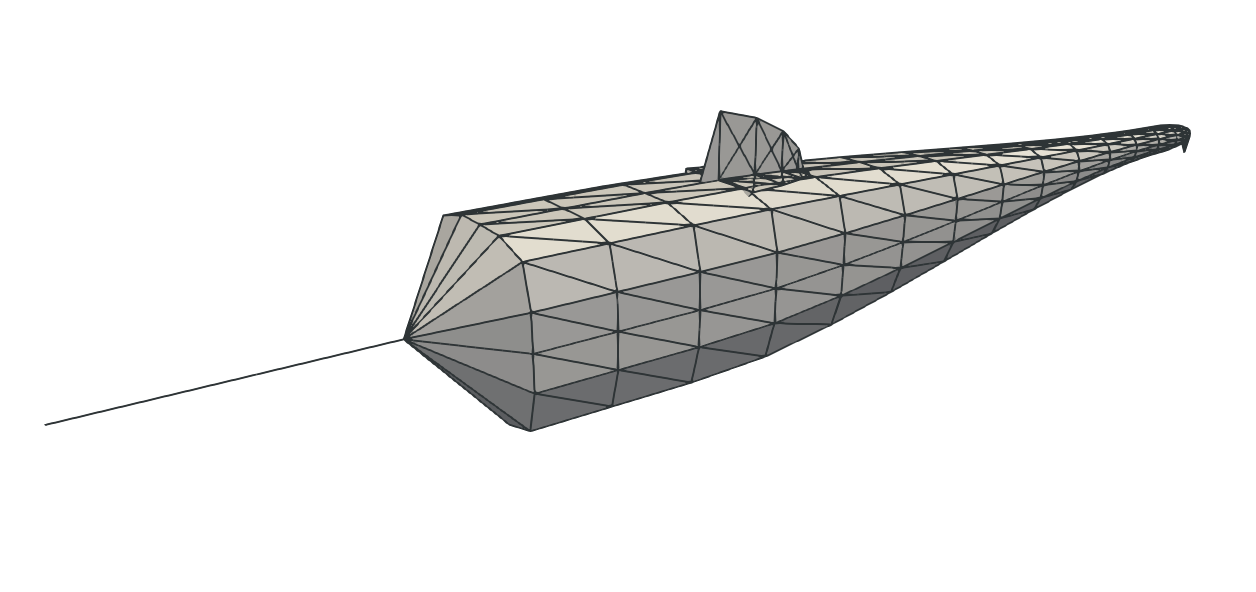
\includegraphics[width=2.1in]{img_fige.png}
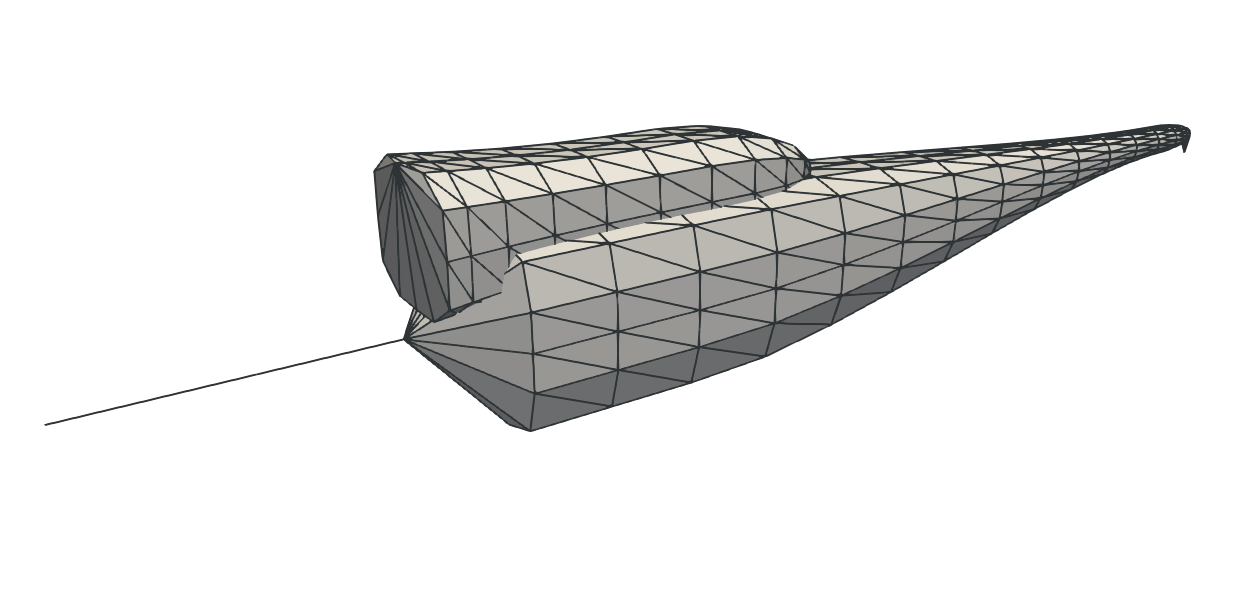
\includegraphics[width=2.1in]{img_figf.png}
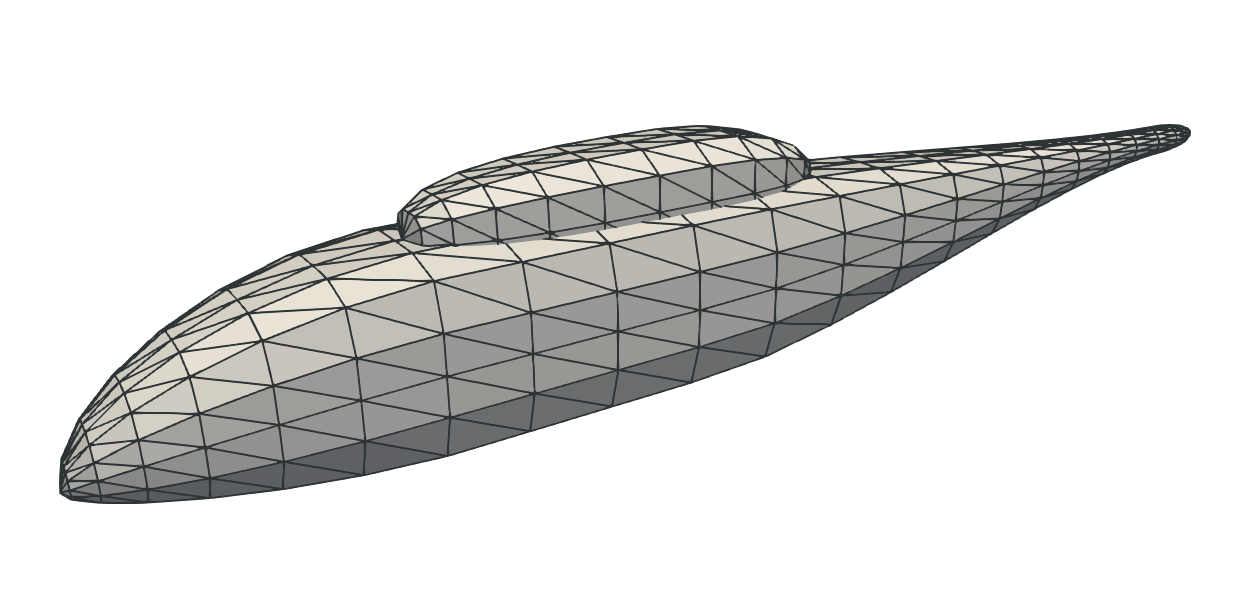
\includegraphics[width=2.1in]{img_figg.png}
\caption{Fuselage and pylon generated by the following: Ref.~\cite{nasa80051} as written (top left); Ref.~\cite{nasa80051} with absolute values around sine and cosine and converting NaN to 0 (top middle); Ref.~\cite{nasa87762} converting NaN to 0 (top right); Ref.~\cite{nasa87762} with sine and NaN fixes (bottom left); Ref.~\cite{mineckgorton} with fixes from Ref.~\cite{nasa87762} and sine and NaN (bottom middle); present work (bottom right).}
\label{allforms}
\end{centering}\end{figure}%
This Technical Note serves as a notice of correct and clarified formulae and coefficients
suitable for automatic calculation.
It also provides a link to a public repository for a program which generates a correct
triangular mesh surface of the ROBIN body \cite{robinsurfmesh}, otherwise unavailable online.
Note that our aim is simply to \emph{allow} generation of the shape as used in previous research,
alleviating any modeling burden on future researchers,
and not to change the intent of the original coefficients, or create a new or different shape.

% --------------------------------------------------------------------------

\section{Method and Proposed Changes}
In proper form, the superellipse function used to define the ROBIN body is
\begin{equation}
   y=r \sin \theta \quad , \quad z=r \cos \theta +Z0
\end{equation} 
where
\begin{equation}
  %r=\left(\frac{\left(\frac{HW}{4}\right)^{N}}{\left(\frac{H}{2}\sin(\theta)\right)^{N}+\left(\frac{W}{2}\cos(\theta)\right)^{N}}\right)^{\frac{1}{N}} \quad \theta\in[0,2\pi].
  r=\left(\frac{\left(\frac{HW}{4}\right)^{N}}{|\frac{H}{2}\sin \theta|^{N}+|\frac{W}{2}\cos \theta|^{N}}\right)^{\frac{1}{N}} \quad \theta\in[0,2\pi].
\label{supell}
\end{equation}
and $H, \ W, \ N$, and $Z0$ are all calculated from
\begin{equation}
  F\!\left(x\right) = C_{6}+C_{7}\left[C_{1}+C_{2}\left(\frac{x+C_{3}}{C_{4}}\right)^{C_{5}}\right]^{\frac{1}{C_{8}}}
\label{coeff}
\end{equation}
with appropriate parameters $C_{1 \to 8}$.
Original \cite{nasa80051} and subsequent \cite{nasa87762} papers confusingly point to different equations
for $N$ and $Z0$.
In addition, all previous authors omit the absolute value modifiers on sine and cosine in Eq.~(\ref{supell}); these are
required to prevent floating point errors when an otherwise negative number is raised to a non-integer power.  
All subsequent corrections involve the coefficients.

Tables \ref{fuscoeff} and \ref{pycoeff} present our proposed coefficients, with changes from the original \cite{nasa80051}
in bold, accounting for all corrections listed below.
%in bold, accounting for all necessary corrections, adjustments for simplicity, and using the pylon from Mineck and
%Gorton (2000) \cite{mineckgorton}.
%\begin{table}[ht]
\begin{table}[!h]
\caption{Coefficients for the fuselage; changes are in \textbf{bold}}
\centering
\begin{tabular}{cccccccccc}
Function & $x$ & $C_{1}$ & $C_{2}$ & $C_{3}$ & $C_{4}$ & $C_{5}$ & $C_{6}$ & $C_{7}$ & $C_{8}$ \\
\hline
$H$          & [0.0, 0.4]  & 1.0 & -1.0 & -0.4 & \textbf{-0.4} & 1.8 & 0.0    & 0.25 & 1.8 \\
$W$          &             & 1.0 & -1.0 & -0.4 & \textbf{-0.4} & 2.0 & 0.0    & 0.25 & 2.0 \\
$Z0$ &                & 1.0 & -1.0 & -0.4 & \textbf{-0.4} & 1.8 & -0.08 & 0.08 & 1.8 \\
$N$           &            & 2.0 & 3.0  & 0.0  &              0.4  & 1.0 & 0.0    & 1.0   & 1.0 \\
\hline
$H$          & [0.4, 0.8]  & \textbf{0.0} & 0.0 & 0.0 & \textbf{1.0} & 0.0 & \textbf{0.25} & 0.0 & \textbf{1.0} \\
$W$          &             & \textbf{0.0} & 0.0 & 0.0 & \textbf{1.0} & 0.0 & \textbf{0.25} & 0.0 & \textbf{1.0} \\
$Z0$ &                & \textbf{0.0} & 0.0 & 0.0 & \textbf{1.0} & 0.0 & 0.0               & 0.0 & \textbf{1.0} \\
$N$           &            & \textbf{0.0} & 0.0 & 0.0 & \textbf{1.0} & 0.0 & \textbf{5.0}   & 0.0 & \textbf{1.0} \\
\hline
$H$          & [0.8, 1.9]  & 1.0 & -1.0 & -0.8 & 1.1 & 1.5 & 0.05 & 0.2 & 0.6 \\
$W$          &             & 1.0 & -1.0 & -0.8 & 1.1 & 1.5 & 0.05 & 0.2 & 0.6 \\
$Z0$ &                & 1.0 & -1.0 & -0.8 & 1.1 & 1.5 & 0.04 & -0.04 & 0.6 \\
$N$           &            & 5.0 & -3.0 & -0.8 & 1.1 & 1.0 & 0.0 & \textbf{1.0} & \textbf{1.0} \\
\hline
$H$          & [1.9, 2.0]  & 1.0 & -1.0 & -1.9 & 0.1 & 2.0 & 0.0 & 0.05 & 2.0 \\
$W$          &             & 1.0 & -1.0 & -1.9 & 0.1 & 2.0 & 0.0 & 0.05 & 2.0 \\
$Z0$ &                & \textbf{0.0} & 0.0 & 0.0 & \textbf{1.0} & 0.0 & \textbf{0.04} & 0.0 & \textbf{1.0} \\
$N$           &            & \textbf{0.0} & 0.0 & 0.0 & \textbf{1.0} & 0.0 & \textbf{2.0} & 0.0 & \textbf{1.0} \\
\end{tabular}
%\vspace{0.1in}
\label{fuscoeff}
\end{table}
\begin{table}[!h]
\caption{Coefficients for the pylon; changes are in \textbf{bold}}
\centering
\begin{tabular}{cccccccccc}
Function & $x$ & $C_{1}$ & $C_{2}$ & $C_{3}$ & $C_{4}$ & $C_{5}$ & $C_{6}$ & $C_{7}$ & $C_{8}$ \\
\hline
$H$          & [0.4, 0.8]  & 1.0             & -1.0 & -0.8 & \textbf{-0.4} & 3.0 & 0.0                  & \textbf{0.145} & 3.0 \\
$W$          &                 & 1.0             & -1.0 & -0.8 & \textbf{-0.4} & 3.0 & 0.0                  & \textbf{0.166} & 3.0 \\
$Z0$ &                 & \textbf{0.0} & 0.0  & 0.0  & \textbf{1.0}  & 0.0  & \textbf{0.125} & 0.0                 & \textbf{1.0} \\
$N$           &                 & \textbf{0.0} & 0.0  & 0.0  & \textbf{1.0}  & 0.0  & \textbf{5.0}     & 0.0                 & \textbf{1.0} \\
\hline
$H$          & [0.8, 1.018]  & 1.0             & -1.0 & -0.8 & 0.218         & 2.0 & 0.0                 & \textbf{0.145} & 2.0 \\
$W$          &                     & 1.0             & -1.0 & -0.8 & 0.218         & 2.0 & 0.0                 & \textbf{0.166} & 2.0 \\
$Z0$ &                     & 1.0             & -1.0 & -0.8 & 1.1             & 1.5 & 0.065             & 0.06               & 0.6 \\
$N$           &                     & \textbf{0.0} & 0.0  & 0.0  & \textbf{1.0} & 0.0 & \textbf{5.0}     & 0.0                 & \textbf{1.0} \\
\end{tabular}
%\vspace{0.1in}
\label{pycoeff}
\end{table}

When applied using the full Eq.~(\ref{coeff}) in an automatic system, the original coefficients result in
frequent floating point errors, which prevent obtaining the correct values for $r$ and $Z0$ and thus $y$ and $z$.
Previous authors had made corrections to alleviate some of these errors (see Fig.~\ref{allforms}), but not all.
%The corrections are summarized below.
\begin{itemize}
\item Two obvious typographic errors in the original \cite{nasa80051} --- $Z0$ in the second body segment and $N$
on the pylon aft --- were caught by later authors \cite{nasa87762,mineckgorton}, but no author reported both.
\item Phelps \& Berry \cite{nasa87762} noted that sections with $C_1$ representing the constant value were raised
to the power of $\frac{1}{C_8} = \frac{1}{0}$ and then multiplied by $C_7 = 0$. They subsequently report using
$C_7 = C_8 = 1$ to correct this.
\end{itemize}

%\begin{figure} \begin{centering}
%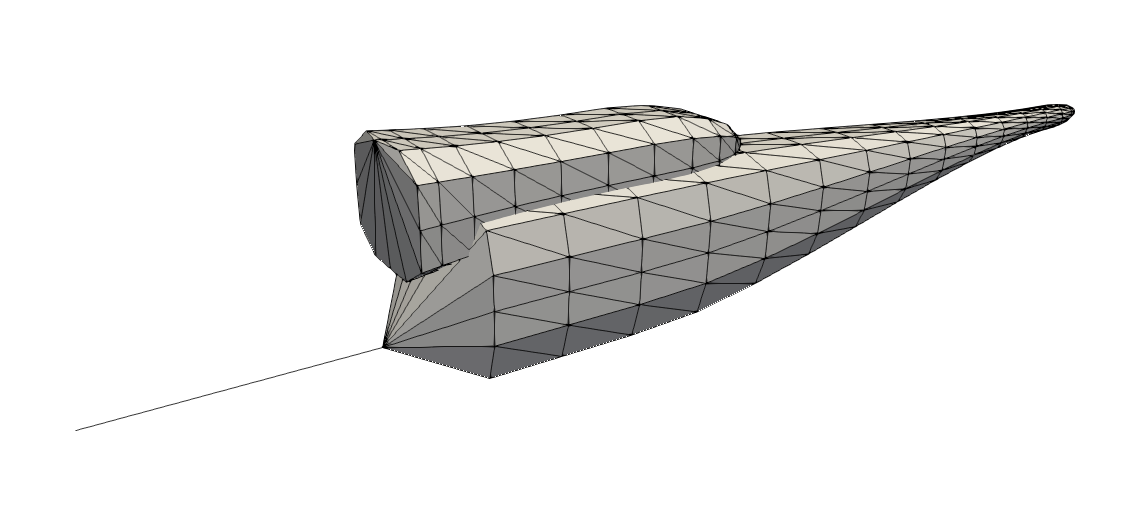
\includegraphics[width=3.0in]{img_badc4.png}
%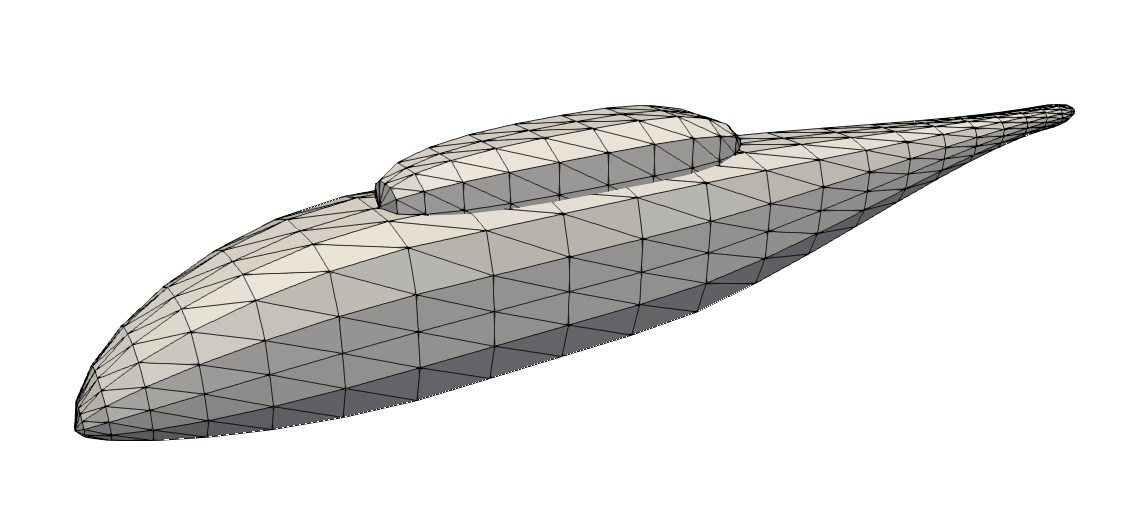
\includegraphics[width=3.0in]{img_good.png}
%\caption{Shape using original positive 4th coefficient (left), shape using correct sign (right).}
%\label{badc4}
%\end{centering}\end{figure}%

Incorporating the corrections from subsequent authors still does not allow creation of the correct shape.
Here we describe further changes to the coefficients that needed to be made.
\begin{itemize}
\item Denominators $C_{4}$ for $H$ and $W$ for the front section of both the fuselage and pylon, as well as $Z0$ for the
front of the fuselage, had the wrong sign and created incorrect results (see Fig.~\ref{allforms}, bottom center and right).
\item In cases where $C_{2}=0$, $C_{4}$ was changed from 0 to 1 to prevent division by zero.
\end{itemize}

%\item Parameters in $C_{1}$ were often multiplied by 0 in $C_{7}$ where they were intended as the resulting values.
%\item On segments with constant values for $F$($x$), the original authors placed the constant value in $C_{1}$,
%which was then multiplied by $C_{7} = 0$.
%\item On segments with constant values for $F$($x$), the original authors placed the constant value in $C_{1}$
%and maintained $C_{2...8} = 0$, which breaks the calculation.
%These single-valued parameters are more clear when they appear as the outermost constant $C_{6}$.
%We moved these constant values from $C_{1}$ to $C_{6}$.

%While the above corrections were necessary to generate a valid shape, there exists in the literature a variation
%of the size of the pylon, defined by coefficients $C_{7}$ for $H$ and $W$.
While the above corrections were necessary to generate a valid shape, the original coefficients generated a 
tall pylon that did not appear to match the model used in those experiments \cite{nasa80051,nasa87762}.
%Values guiding the shape of the pylon ($C_{7}$) differ between earlier and later works.
We thus use coefficients $C_{7}$ for $H$ and $W$ from Mineck and Gorton (2000) \cite{mineckgorton}.
%This was recognized by Mineck and Gorton (2000) \cite{mineckgorton}, whose coefficients $C_{7}$ for $H$ and $W$
%we use.
%We have chosen to use values from Mineck and Gorton (2000) \cite{mineckgorton} because the shape of the generated 
%pylon matches the photos and drawings from earlier papers more closely \cite{nasa80051,nasa87762} than the original coefficients.
Figure \ref{badpylon} shows both original ($C_{7,H} = 0.2$, $C_{7,W} = 0.172$) and
updated ($C_{7,H} = 0.145$, $C_{7,W} = 0.166$) pylon shapes.
\begin{figure} \begin{centering}
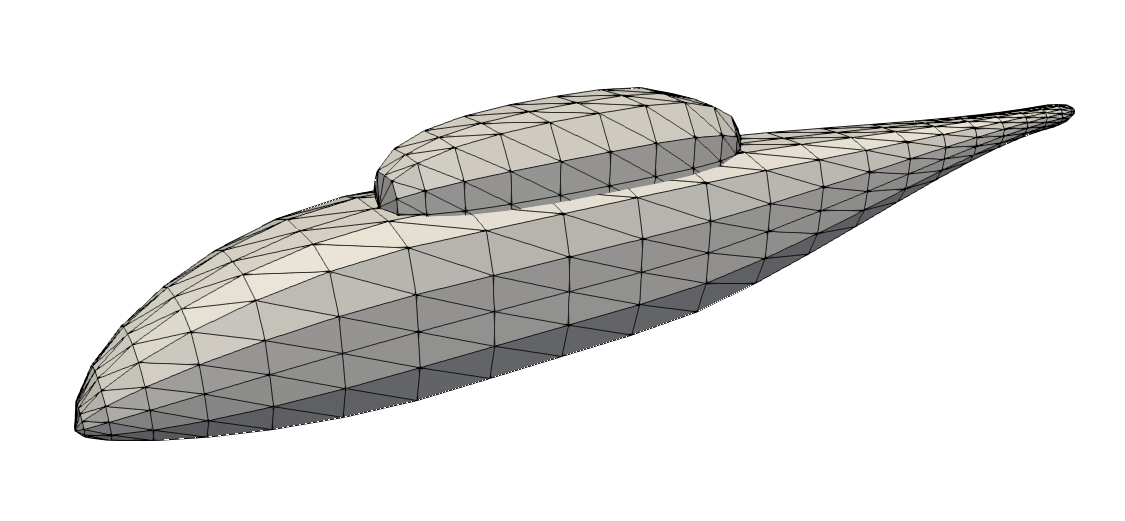
\includegraphics[width=3.0in]{img_badpylon.png}
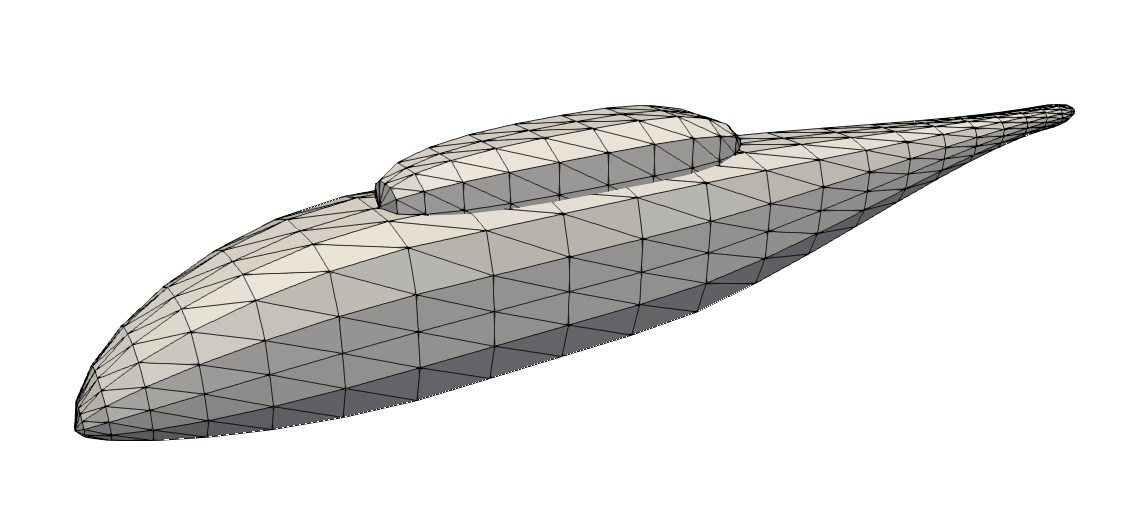
\includegraphics[width=3.0in]{img_good.png}
%\vspace{0.1in}
\caption{Pylon using original coefficients \cite{nasa80051,nasa87762} (left), pylon from Mineck and Gorton (2000) \cite{mineckgorton} (right).}
\label{badpylon}
\end{centering}\end{figure}%

A final change reported in the coefficients in Tables \ref{fuscoeff} and \ref{pycoeff} represents a preference
for simplicity and is not required for correctness.
Coefficient sets that were intended to produce a constant value over the interval placed the constant value in $C_1$,
inside the brackets in Eq.~\ref{coeff}. In order to avoid floating point errors, this requires also setting
$C_4 = C_7 = C_8 = 1$. Alternatively, if that constant value were assigned to $C_6$, outside the brackets, one only
needs to set $C_4 = C_8 = 1$ to achieve the desired result.


Portable C++ code using these formulae and coefficients is provided at the following Github link:
\url{https://github.com/Applied-Scientific-Research/robin-surface-mesh} \cite{robinsurfmesh}.
The compiled program generates a triangular mesh with a user-specified number of nodes across
the length and circumference of the fuselage and pylon.


% --------------------------------------------------------------------------
\section{Conclusion}

This Technical Note contains corrected coefficients and robust formulae for
easy reproduction of the ROBIN body, a well-studied but erratically documented
geometry useful for studies of rotary-wing aerodynamics.
The equations are now easily translatable to a computer algorithm, and an
open-source program which recreates the surface geometry has been created.
We hope that future research projects will not be led astray by past 
inconsistencies in the reporting of the body coefficients and formulae.


% --------------------------------------------------------------------------
%\bibliographystyle{abbrv}
\bibliography{robinbib}
%--------------------------------------------------------------------------- 

\end{document}
